\documentclass{article}

\usepackage{graphicx}
\usepackage{tikz}
\usepackage{tikzsymbols}
\usetikzlibrary{calc,patterns,shapes.geometric}
\pagestyle{empty}
\usepackage[margin=0pt]{geometry}
\geometry{papersize={14in,12in}}

\def\centerarc[#1](#2)(#3:#4:#5){\draw[#1] ($(#2)+({#5*cos(#3)},{#5*sin(#3)})$) arc (#3:#4:#5);}

\begin{document}
	\begin{figure}
		\centering
		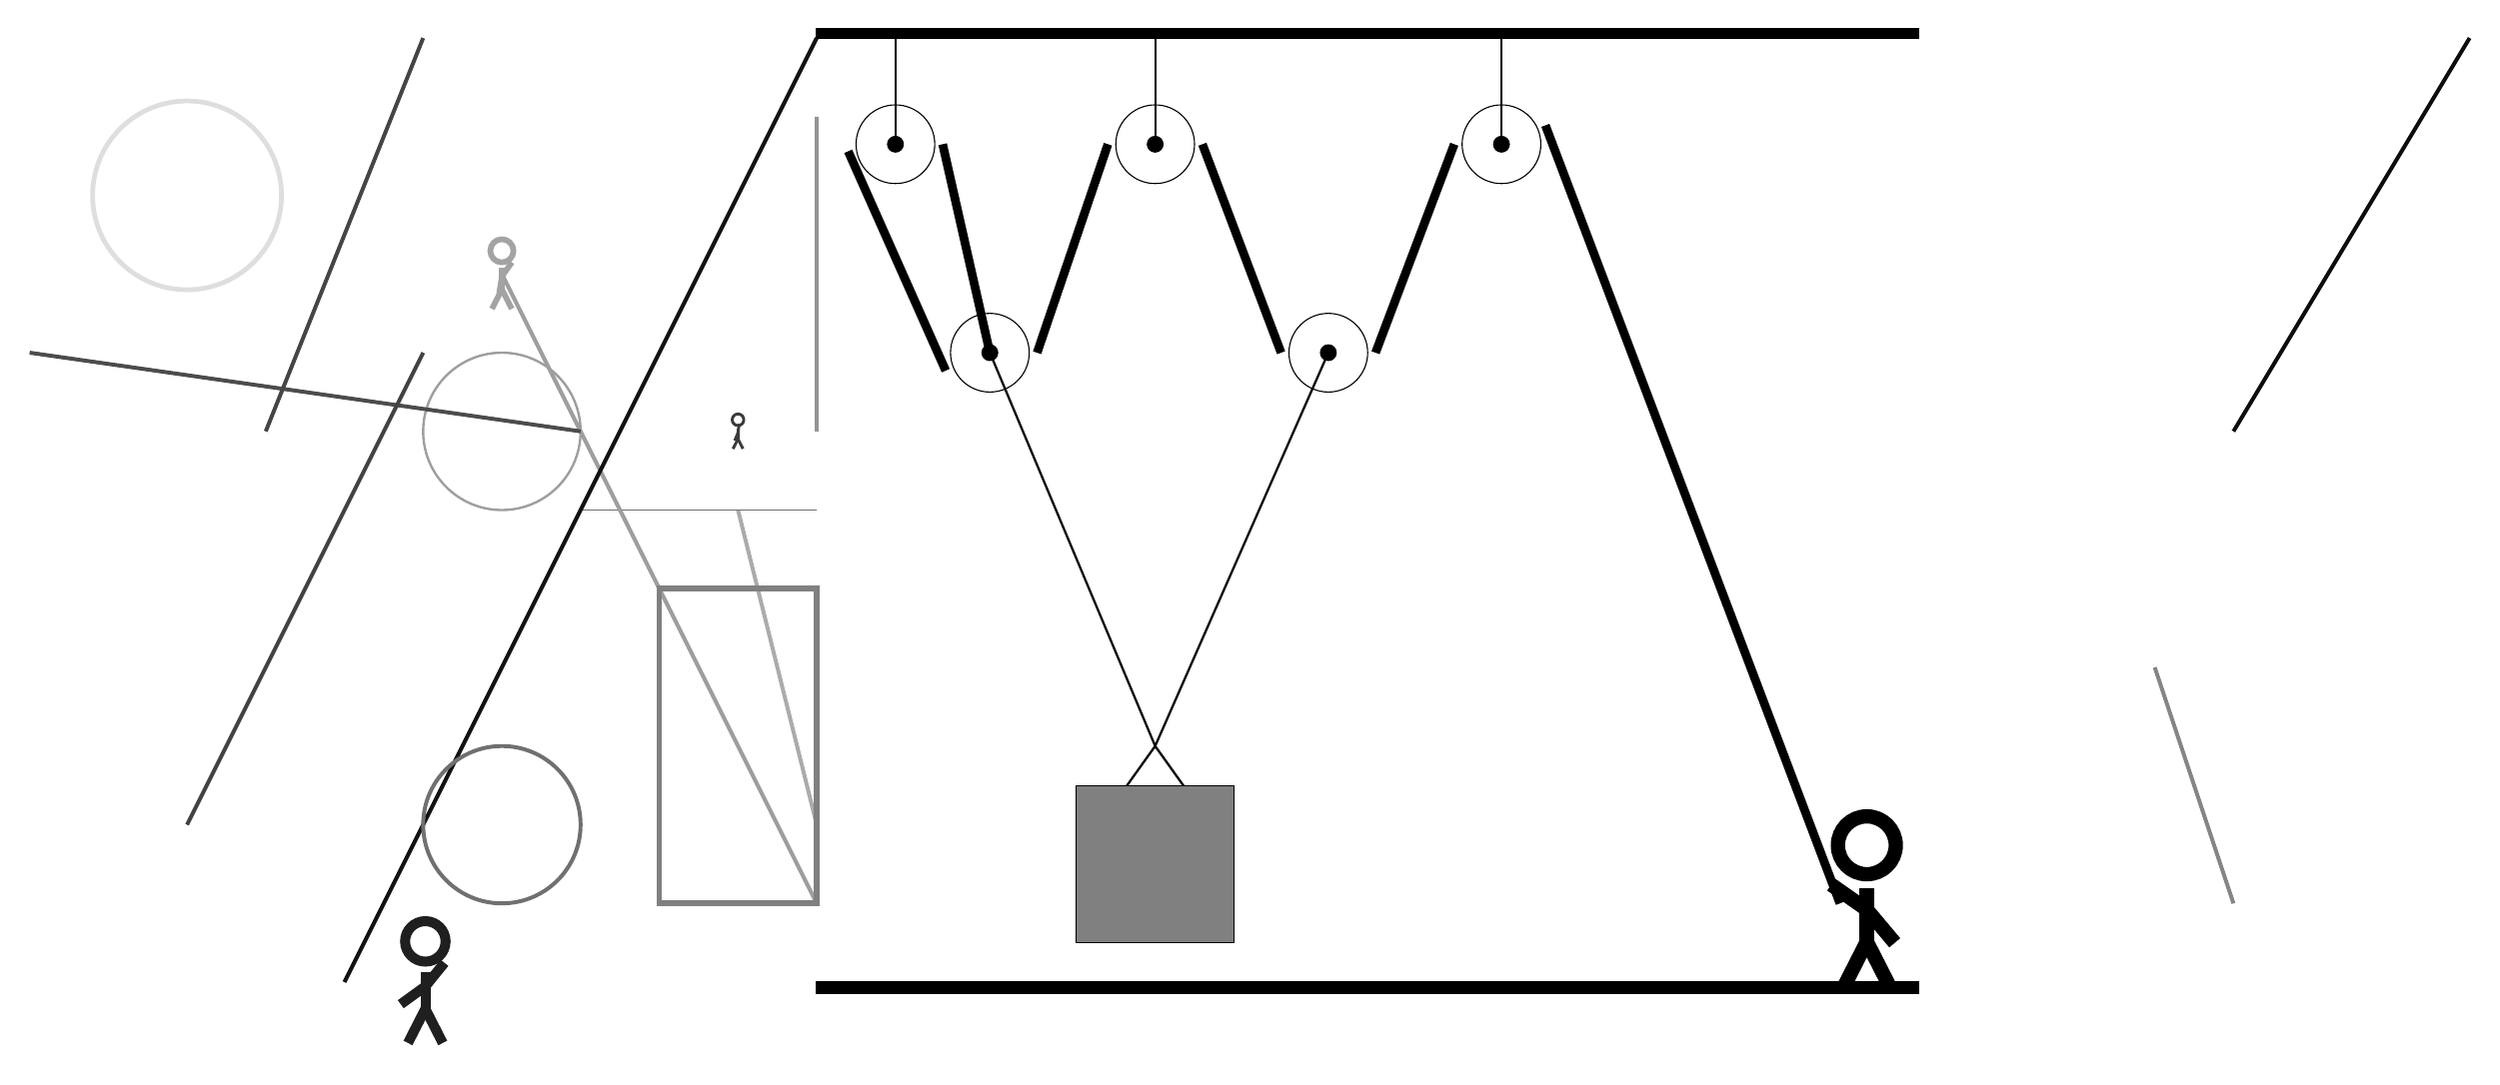
\begin{tikzpicture}
			%%%%% START %%%%%
			
			\draw[fill=black] (-2, 9) rectangle (12, 9.125);
			
			\draw (-1, 7.65) circle (0.5);
			\draw[fill=black] (-1, 7.65) circle (0.1);
			\draw[thick] (-1, 7.65) -- (-1, 9);
			
			\draw (2.3, 7.65) circle (0.5);
			\draw[fill=black] (2.3, 7.65) circle (0.1);
			\draw[thick] (2.3, 7.65) -- (2.3, 9);
			
			\draw (6.7, 7.65) circle (0.5);
			\draw[fill=black] (6.7, 7.65) circle (0.1);
			\draw[thick] (6.7, 7.65) -- (6.7, 9);
			
			\draw (0.2, 5) circle (0.5);
			\draw[fill=black] (0.2, 5) circle (0.1);
			
			\draw (4.5, 5) circle (0.5);
			\draw[fill=black] (4.5, 5) circle (0.1);
			
			\draw[thick] (0.2, 5) -- (2.3, 0)  -- (4.5, 5);
			\draw[thick]  (1.8, -0.7) -- (2.3, 0) -- (2.8, -0.7);
			\draw[fill=black!50] (1.3, -0.5) rectangle (3.3, -2.5);
			
			\draw[line width=1.1mm] (0.2, 5) -- (-0.4, 7.65);
			\centerarc[line width=1.1mm](-1, 7.65)(0:200:0.6);
			\draw[line width=1.1mm] (-1.6, 7.56) -- (-0.361, 4.772);
			\centerarc[line width=1.1mm](0.2, 5)(200:360:0.6);
			\draw[line width=1.1mm](0.8, 5) -- (1.7, 7.65);
			\centerarc[line width=1.1mm](2.3, 7.65)(0:180:0.6);
			\draw[line width=1.1mm] (2.9, 7.65) -- (3.9, 5);
			\centerarc[line width=1.1mm](4.5, 5)(180:360:0.6);
			\draw[line width=1.1mm] (5.1, 5) -- (6.1, 7.65);
			\centerarc[line width=1.1mm](6.7, 7.65)(20:180:0.6);
			\draw[line width=1.1mm](7.258, 7.89)  -- (11, -2);
			
			\node at (11.3, -2) {\Strichmaxerl[10][-35][-50]};
			
			\draw[line width=0.5mm, color=black!33](-2, -1) -- (-3, 3);
			
			\draw[line width=0.4mm, color=black!42] (-2, 4) rectangle (-2, 8);
			\node[line width=0.4mm, color=black!77] at (-3, 4) {\Strichmaxerl[2][68][82]};
			\draw[line width=0.2mm, color=black!57] (-2, 3) rectangle (-5, 3);
			\draw[line width=0.5mm, color=black!38](-6, 6) -- (-2, -2);
			
			\draw[line width=0.5mm, color=black!95](16, 4) -- (19, 9);
			
			\node[line width=0.3mm, color=black!88] at (-7, -3) {\Strichmaxerl[7][36][51]};
			
			\draw[line width=0.5mm, color=black!48](15, 1) -- (16, -2);
			\draw [line width=0.3mm, color=black!38](-6, 4) circle (1.0);
			\node[line width=0.7mm, color=black!36] at (-6, 6) {\Strichmaxerl[4][81][55]};
			\draw [line width=0.6mm, color=black!13](-10, 7) circle (1.2);
			\draw[line width=0.5mm, color=black!93](-2, 9) -- (-8, -3);
			\draw[line width=0.7mm, color=black!50] (-2, -2) rectangle (-4, 2);
			
			\draw[line width=0.5mm, color=black!70](-5, 4) -- (-12, 5);
			\draw [line width=0.5mm, color=black!56](-6, -1) circle (1.0);
			\draw[line width=0.5mm, color=black!73](-7, 9) -- (-9, 4);
			
			\draw[line width=0.5mm, color=black!74](-7, 5) -- (-10, -1);
			
			\draw[fill=black] (-2, -3) rectangle (12, -3.15);
			
			%%%%% END %%%%%
		\end{tikzpicture}
	\end{figure}	
\end{document}